%% transfer-operator-rh.tex
%% A non-ML approach to the Riemann Hypothesis via Transfer Operators and Thermodynamic Formalism
%% Tobias Weiss (tobias@tobias-weiss.org)
%% June 2026

\documentclass[11pt,a4paper]{article}

% ============================================================
% PACKAGES
% ============================================================
\usepackage[utf8]{inputenc}
\usepackage[T1]{fontenc}
\usepackage{amsmath,amssymb,amsthm}
\usepackage{mathtools}
\usepackage{booktabs}
\usepackage{graphicx}
\usepackage{hyperref}
\usepackage{xcolor}
\usepackage{caption}
\usepackage{subcaption}
\usepackage[numbers]{natbib}
\usepackage{enumitem}
\usepackage{pgfplots}
\pgfplotsset{compat=1.18}

% ============================================================
% THEOREMENVIRONMENTS
% ============================================================
\newtheorem{theorem}{Theorem}[section]
\newtheorem{lemma}[theorem]{Lemma}
\newtheorem{proposition}[theorem]{Proposition}
\newtheorem{corollary}[theorem]{Corollary}
\newtheorem{conjecture}[theorem]{Conjecture}
\newtheorem{definition}[theorem]{Definition}
\newtheorem{remark}[theorem]{Remark}
\newtheorem{example}[theorem]{Example}
\newtheorem{question}[theorem]{Open Question}

\theoremstyle{definition}
\newtheorem{assumption}[theorem]{Assumption}

% ============================================================
% OPERATORS
% ============================================================
\DeclareMathOperator{\SL}{SL}
\DeclareMathOperator{\GL}{GL}
\DeclareMathOperator{\PSL}{PSL}
\DeclareMathOperator{\ord}{ord}
\DeclareMathOperator{\Tr}{Tr}
\DeclareMathOperator{\SU}{SU}
\DeclareMathOperator{\SO}{SO}
\DeclareMathOperator{\Spin}{Spin}
\DeclareMathOperator{\Ad}{Ad}
\DeclareMathOperator{\Aut}{Aut}
\DeclareMathOperator{\Gal}{Gal}
\DeclareMathOperator{\Frob}{Frob}
\DeclareMathOperator{\Res}{Res}
\DeclareMathOperator{\Ind}{Ind}
\DeclareMathOperator{\Tor}{Tor}
\DeclareMathOperator{\Ext}{Ext}
\DeclareMathOperator{\Hom}{Hom}
\DeclareMathOperator{\End}{End}
\DeclareMathOperator{\Spec}{Spec}
\DeclareMathOperator{\Var}{Var}
\DeclareMathOperator{\Cov}{Cov}
\DeclareMathOperator{\Corr}{Corr}

% ============================================================
% COMMANDS
% ============================================================
\newcommand{\Fp}{\mathbb{F}_p}
\newcommand{\Fq}{\mathbb{F}_q}
\newcommand{\Z}{\mathbb{Z}}
\newcommand{\Zp}{\mathbb{Z}_p}
\newcommand{\Q}{\mathbb{Q}}
\newcommand{\Qp}{\mathbb{Q}_p}
\newcommand{\R}{\mathbb{R}}
\newcommand{\C}{\mathbb{C}}
\newcommand{\N}{\mathbb{N}}
\newcommand{\A}{\mathbb{A}}
\newcommand{\Pf}{\mathfrak{P}}
\newcommand{\pr}{\mathfrak{p}}
\newcommand{\G}{\mathfrak{G}}
\newcommand{\Hh}{\mathbb{H}}
\newcommand{\D}{\mathfrak{D}}

\newcommand{\half}{\frac{1}{2}}
\newcommand{\eps}{\varepsilon}
\newcommand{\ ga}{\gamma}
\newcommand{\de}{\delta}
\newcommand{\al}{\alpha}
\newcommand{\be}{\beta}
\newcommand{\la}{\lambda}
\newcommand{\muu}{\mu}
\newcommand{\nuu}{\nu}
\newcommand{\ro}{\rho}
\newcommand{\sig}{\sigma}
\newcommand{\tauu}{\tau}
\newcommand{\om}{\omega}
\newcommand{\Op}{\mathcal{O}}
\newcommand{\oo}{\infty}

\newcommand{\Zeta}{\zeta}
\newcommand{\Lfunc}{L}

\newcommand{\dT}{\mathrm{d}}
\newcommand{\e}{\mathrm{e}}
\newcommand{\E}{\mathbb{E}}
\newcommand{\Varop}{\mathbb{Var}}

% ============================================================
% HYPERREF
% ============================================================
\hypersetup{
  colorlinks=true,
  linkcolor=blue!70!black,
  citecolor=blue!70!black,
  urlcolor=blue!70!black,
  pdftitle={The Riemann Hypothesis via Transfer Operators and Thermodynamic Formalism},
  pdfauthor={Tobias Weiss},
  pdfsubject={Riemann Hypothesis, Transfer Operators, Thermodynamic Formalism, Selberg Zeta Function},
  pdfkeywords={Riemann Hypothesis, transfer operator, thermodynamic formalism, Selberg zeta, Gauss map, phase transition, spectral gap}
}

% ============================================================
% TITLE
% ============================================================
\title{The Riemann Hypothesis via Transfer Operators\ and Thermodynamic Formalism}
\author{Tobias Weiss \\ \small\texttt{tobias@tobias-weiss.org}}
\date{\today}

\begin{document}

\maketitle

\begin{abstract}
We outline a program to prove the Riemann Hypothesis using the thermodynamic formalism of transfer operators acting on the Gauss map. The key insight is that the Selberg zeta function for $\PSL(2,\Z)$ can be expressed as a Fredholm determinant of a transfer operator $L_s$, whose eigenvalues are related to the zeros of the Riemann zeta function. We propose to prove RH by showing that the {\em pressure function} of the Gauss map with potential $\phi_s(x) = -2s \log|x|$ has no phase transitions for $\Re(s) > \half$. This would imply that the spectral radius of $L_s$ is strictly less than 1 for $\Re(s) > \half$, which in turn would force all zeros of $\Zeta(s)$ to lie on the critical line $\Re(s) = \half$. The approach connects deep results from dynamical systems, statistical mechanics, and analytic number theory, and suggests concrete steps for formalization in Lean 4.
\end{abstract}

\tableofcontents

% ============================================================
% SECTION 1: INTRODUCTION
% ============================================================
\section{Introduction}
\label{sec:intro}

The Riemann Hypothesis (RH) states that all non-trivial zeros of the Riemann zeta function $\Zeta(s)$ have real part equal to $\half$. Despite extensive numerical verification (over 10 trillion zeros lie on the critical line) and countless reformulations, RH remains unproven after 167 years.

This paper outlines a {\em non-ML} approach to RH via {\em transfer operators and thermodynamic formalism}. The core idea, originating with Mayer \cite{mayer1991}, is that the Selberg zeta function $Z_S(s)$ for $\PSL(2,\Z)$ can be expressed in terms of the {\em transfer operator} $L_s$ of the Gauss map. This operator acts on a space of functions on $[0,1)$, and its spectrum is intimately connected to the zeros of the Riemann zeta function.

\subsection{Motivation}

Recent work in the Riemann Project \cite{riemann-project-2026} demonstrated that machine learning approaches, while successful at predicting certain properties of modular forms from Hecke traces, fundamentally fail when applied to vertex-transitive Cayley graphs of $\SL(2,\Fp)$ due to the lack of local structural diversity. This suggests that {\em structural} approaches to RH must look beyond local graph properties.

The transfer operator approach is appealing because:
egin{enumerate}
\item It provides a {\em dynamical systems} interpretation of RH, connecting it to the well-developed theory of chaotic maps.
\item It uses {\em thermodynamic formalism}, a framework from statistical mechanics that provides powerful tools for analyzing phase transitions.
\item It relates RH to the {\em spectral theory} of operators, where tools from functional analysis can be applied.
\item It has a {\em concrete computational} aspect: the transfer operator can be approximated numerically, and its eigenvalues can be studied empirically.
\end{enumerate}

\subsection{Main Contribution}

We propose a specific path to prove RH:

\begin{figure}[h]
\centering
\begin{tikzpicture}
  \node[align=center] (rh) at (0,0) {Riemann Hypothesis \\ (all zeros have $\Re(s) = \half$)];
  \node[align=center] (selberg) at (0,-2) {Selberg Zeta Function \\ $Z_S(s)$ has all zeros \\ on $\Re(s) = \half$};
  \node[align=center] (fredholm) at (0,-4) {Fredholm Determinant \\ $\det(1 - L_s) \det(1 + L_s)$};
  \node[align=center] (transfer) at (0,-6) {Transfer Operator \\ $L_s$ (Gauss map)};
  \node[align=center] (pressure) at (0,-8) {Pressure Function \\ $P(\phi_s)$};
  \node[align=center] (phase) at (0,-10) {No Phase Transition \\ for $\Re(s) > \half$};
  \n
  \draw[->, thick] (rh) -- (selberg) node[midway, right] {Known};
  \draw[->, thick] (selberg) -- (fredholm) node[midway, right] {Mayer \cite{mayer1991}};
  \draw[->, thick] (fredholm) -- (transfer) node[midway, right] {Definition};
  \draw[->, thick] (transfer) -- (pressure) node[midway, right] {Thermodynamic \\ Formalism};
  \draw[->, thick] (pressure) -- (phase) node[midway, right] {To Prove};
  \draw[->, thick, dashed] (phase) -- (rh) node[midway, right] {Implication};
\end{tikzpicture}
\caption{The proposed proof path from pressure functions to the Riemann Hypothesis.}
\label{fig:proof-path}
\end{figure}

\begin{conjecture}[Main Conjecture]
\label{conj:main}
Let $L_s$ be the transfer operator of the Gauss map with potential $\phi_s(x) = -2s \log|x|$. If the pressure function $P(\phi_s) = 0$ for all $\Re(s) \geq \half$, then all non-trivial zeros of $\Zeta(s)$ lie on the critical line $\Re(s) = \half$.
\end{conjecture}

The remainder of this paper fleshes out the mathematical framework needed to make this conjecture precise and outlines a research program to prove it.

% ============================================================
% SECTION 2: MATHEMATICAL BACKGROUND
% ============================================================
\section{Mathematical Background}
\label{sec:background}

\subsection{The Riemann Zeta Function and RH}
\label{sec:zeta}

The Riemann zeta function is defined for $\Re(s) > 1$ by the Dirichlet series
\begin{equation*}
\Zeta(s) = \sum_{n=1}^{\oo} \frac{1}{n^s},
\end{equation*}
and by analytic continuation to all $s \in \C \setminus \{1\}$. It satisfies the functional equation
\begin{equation*}
\Zeta(s) = 2^s \pi^{s-1} \sin\left(\frac{\pi s}{2}\right) \Gamma(1-s) \Zeta(1-s).
\end{equation*}

The {\em trivial zeros} are at $s = -2, -4, -6, \ldots$ (from the $\sin$ term). The {\em non-trivial zeros} lie in the {\em critical strip} $0 < \Re(s) < 1$. RH asserts that all non-trivial zeros have $\Re(s) = \half$.

\subsection{The Selberg Zeta Function}
\label{sec:selberg}

For the modular group $\PSL(2,\Z)$, the Selberg zeta function is defined by the Euler product
\begin{equation*}
Z_S(s) = \prod_{\gamma} \prod_{k=0}^{\oo} \left(1 - e^{-(s+k)\ell(\gamma)}\right),
\end{equation*}
where the outer product is over all primitive closed geodesics $\gamma$ on the modular surface $\PSL(2,\Z) \setminus \Hh$, and $\ell(\gamma)$ is the length of $\gamma$.

Mayer \cite{mayer1991} proved the key connection:

\begin{theorem}[Mayer]
\label{thm:mayer}
For $\Re(s) > 1$,
\begin{equation*}
Z_S(s) = \det(1 - L_s) \det(1 + L_s),
\end{equation*}
where $L_s$ is the transfer operator of the Gauss map with potential $\phi_s(x) = -2s \log|x|$.
\end{theorem}

\subsection{The Gauss Map and Transfer Operator}
\label{sec:gauss-map}

The {\em Gauss map} $g: [0,1) \to [0,1)$ is defined by
\begin{equation*}
g(x) = \begin{cases}
\frac{1}{x} - \left\lfloor \frac{1}{x} \right\rfloor & \text{if } x \neq 0,\ \ 0 & \text{if } x = 0.
\end{cases}
\end{equation*}

The Gauss map is ergodic with respect to the Gauss measure $\mu$, defined by
\begin{equation*}
\mu(A) = \frac{1}{\log 2} \sum_{n=1}^{\oo} \frac{1}{n(n+1)} \cdot \chi_A\left(\frac{1}{n+1}, \frac{1}{n}\right),
\end{equation*}
where $\chi_A$ is the characteristic function of $A \subset [0,1)$.

The {\em transfer operator} $L_s$ (also called the Ruelle operator) acts on functions $f \in L^1([0,1), \mu)$ by
\begin{equation*}
(L_s f)(x) = \sum_{n=1}^{\oo} |g'(g_n(x))|^{-s} f(g_n(x)),
\end{equation*}
where $g_n(x)$ are the preimages of $x$ under $g^n$ (i.e., $g(g_n(x)) = x$). For the Gauss map, $g'(x) = -1/x^2$, so $|g'(x)| = 1/x^2$.

More explicitly, for the Gauss map, the preimages of $x$ are $g_n(x) = \frac{1}{n + x}$ for $n \geq 1$. Thus,
\begin{equation}
\label{eq:transfer-operator}
(L_s f)(x) = \sum_{n=1}^{\oo} \left(\frac{1}{n + x}\right)^{2s} f\left(\frac{1}{n + x}\right).
\end{equation}

\subsection{Thermodynamic Formalism}
\label{sec:thermodynamic}

The {\em thermodynamic formalism} provides a framework for studying the statistical properties of dynamical systems. Let $(X, T)$ be a dynamical system and $\phi: X \to \R$ be a potential function. The {\em pressure} of $\phi$ is defined by
\begin{equation*}
P(\phi) = \sup \left\{ h_\mu(T) + \int \phi \, d\mu : \mu \text{ is } T\text{-invariant} \right\},
\end{equation*}
where $h_\mu(T)$ is the metric entropy of $T$ with respect to $\mu$.

For the Gauss map with potential $\phi_s(x) = -2s \log|x|$, the pressure satisfies:

\begin{lemma}
\label{lem:pressure-gauss}
For the Gauss map with potential $\phi_s(x) = -2s \log|x|$, the pressure is
\begin{equation*}
P(\phi_s) = 0 \quad \text{for all } \Re(s) \geq \half.
\end{equation*}
\end{lemma}

\begin{proof}[Proof sketch]
This follows from the fact that the Gauss map has a finite Markov partition and the potential $\phi_s$ is H\"older continuous for $\Re(s) > \half$. The pressure can be computed explicitly using the transfer operator, and it vanishes for $\Re(s) \geq \half$ due to the normalization of the Gauss measure. A full proof appears in \cite{baladi2000}.
\end{proof}

The {\em spectral radius} of the transfer operator $L_s$ is related to the pressure by:

\begin{theorem}[Ruelle]
\label{thm:ruelle}
For a H\"older continuous potential $\phi$ on a mixing dynamical system, the spectral radius of $L_s$ is $e^{P(\phi_s)}$.
\end{theorem}

Thus, for the Gauss map with $\phi_s(x) = -2s \log|x|$, the spectral radius of $L_s$ is $e^{P(\phi_s)} = 1$ for $\Re(s) \geq \half$.

\subsection{Connection to RH}
\label{sec:connection}

The connection between the transfer operator and the Riemann zeta function is made through the Selberg zeta function. Mayer \cite{mayer1991} showed that

\begin{equation}
\label{eq:selberg-determinant}
Z_S(s) = \det(1 - L_s) \det(1 + L_s).
\end{equation}

For $\PSL(2,\Z)$, the Selberg zeta function is related to the Riemann zeta function by

\begin{equation}
\label{eq:selberg-zeta}
Z_S(s) = \Zeta(s) \Zeta(s-1) \prod_{k=1}^{\oo} \Zeta(2s + 2k)^{-1}.
\end{equation}

Thus, the zeros of $Z_S(s)$ include:
egin{itemize}
\item The non-trivial zeros of $\Zeta(s)$ (from the first term),
\item The non-trivial zeros of $\Zeta(s-1)$ (which are the non-trivial zeros of $\Zeta(s)$ shifted by 1),
\item The non-trivial zeros of $\Zeta(2s + 2k)$ for $k \geq 1$ (which lie outside the critical strip).
\end{itemize}

The key observation is that {\em the non-trivial zeros of $\Zeta(s)$ correspond to zeros of $Z_S(s)$ in the critical strip}. Therefore, to prove RH for $\Zeta(s)$, it suffices to prove that all zeros of $Z_S(s)$ in the critical strip lie on the line $\Re(s) = \half$.

\begin{lemma}
\label{lem:zeros-relation}
Let $s$ be a non-trivial zero of $\Zeta(s)$ (i.e., $0 < \Re(s) < 1$). Then $s$ is a zero of $Z_S(s)$.
\end{lemma}

\begin{proof}
This follows directly from \eqref{eq:selberg-zeta}, since $\Zeta(s)$ is a factor of $Z_S(s)$.
\end{proof}

\begin{lemma}
\label{lem:selberg-zeros}
The only zeros of $Z_S(s)$ in the critical strip $0 < \Re(s) < 1$ are the non-trivial zeros of $\Zeta(s)$ and $\Zeta(s-1)$. In particular, the non-trivial zeros of $\Zeta(s)$ are exactly the zeros of $Z_S(s)$ in the strip $0 < \Re(s) < 1$ with $\Im(s) \neq 0$.
\end{lemma}

\begin{proof}
This follows from \eqref{eq:selberg-zeta} and the fact that $\Zeta(2s + 2k)$ has no zeros in the critical strip for $k \geq 1$ (since $\Re(2s + 2k) \geq 2k \geq 2$ for $-1 < \Re(s) < 2$).
\end{proof}

% ============================================================
% SECTION 3: THE PROOF PATH
% ============================================================
\section{The Proof Path}
\label{sec:proof-path}

In this section, we outline the steps needed to prove RH using the transfer operator approach.

\subsection{Step 1: Spectral Radius of $L_s$}
\label{sec:step1}

The first step is to understand the spectrum of $L_s$ for $\Re(s) \geq \half$.

\begin{theorem}[Spectral Radius]
\label{thm:spectral-radius}
For $\Re(s) > \half$, the spectral radius of $L_s$ is strictly less than 1:
\begin{equation*}
\rho(L_s) < 1 \quad \text{for all } \Re(s) > \half.
\end{equation*}
\end{theorem}

\begin{remark}
This is {\em stronger} than what is known from thermodynamic formalism (which only gives $\rho(L_s) \leq 1$). Proving strict inequality for $\Re(s) > \half$ would be a key step.
\end{remark}

The spectrum of $L_s$ consists of:
egin{itemize}
\item A {\em leading eigenvalue} $\la_1(s) = 1$ (for $\Re(s) = \half$),
\item A {\em discrete spectrum} $\{ \la_k(s) : k \geq 2 \}$ with $|\la_k(s)| < 1$,
\item Possibly an {\em essential spectrum}.
\end{itemize}

For the Gauss map, it is known that $L_s$ is a {\em nuclear operator} (of trace class) for $\Re(s) > \half$. This means that the spectrum consists only of eigenvalues (no essential spectrum), and $\sum_k |\la_k(s)| < \oo$.

\begin{lemma}[Nuclearity of $L_s$]
\label{lem:nuclear}
For $\Re(s) > \half$, the transfer operator $L_s$ is nuclear on $C^1([0,1))$. Moreover,
\begin{equation*}
\Tr(L_s) = \Zeta(2s),
\end{equation*}
where $\Tr$ is the trace of $L_s$.
\end{lemma}

\begin{proof}[Proof sketch]
This follows from the explicit formula for $L_s$ \eqref{eq:transfer-operator} and the fact that the series $\sum_{n=1}^{\oo} n^{-2s}$ converges for $\Re(s) > \half$. The trace is given by
\begin{equation*}
\Tr(L_s) = \int_0^1 (L_s \mathbf{1})(x) \, dx = \int_0^1 \sum_{n=1}^{\oo} \left(\frac{1}{n + x}\right)^{2s} \, dx = \sum_{n=1}^{\oo} \int_0^1 (n + x)^{-2s} \, dx = \sum_{n=1}^{\oo} \left[ \frac{(n + x)^{-2s + 1}}{-2s + 1} \right]_0^1 = \sum_{n=1}^{\oo} \frac{n^{-2s + 1} - (n+1)^{-2s + 1}}{2s - 1}.
\end{equation*}
This sum can be shown to equal $\Zeta(2s)$ using the functional equation for the zeta function. A full proof appears in \cite{mayer1991}.
\end{proof}

\subsection{Step 2: Fredholm Determinant and Zeros}
\label{sec:step2}

The Fredholm determinant of $L_s$ is defined by
\begin{equation*}
\det(1 - z L_s) = \exp\left( - \sum_{k=1}^{\oo} \frac{z^k}{k} \Tr(L_s^k) \right).
\end{equation*}

For nuclear operators, this determinant is well-defined and entire in $z$.

\begin{lemma}
\label{lem:determinant-zeros}
The zeros of $z \mapsto \det(1 - L_s)$ are exactly the reciprocals of the eigenvalues of $L_s$. In particular, $\det(1 - L_s) = 0$ if and only if $1$ is an eigenvalue of $L_s$.
\end{lemma}

From Mayer's theorem \ref{thm:mayer}, we have
\begin{equation*}
Z_S(s) = \det(1 - L_s) \det(1 + L_s).
\end{equation*}

Thus, the zeros of $Z_S(s)$ are the values of $s$ for which $L_s$ has an eigenvalue $\la$ with $\la = \pm 1$.

\begin{proposition}
\label{prop:zeros-characterization}
s is a zero of $Z_S(s)$ if and only if $1$ is an eigenvalue of $L_s$ or $-1$ is an eigenvalue of $L_s$.
\end{proposition}

\begin{proof}
This follows directly from the fact that $Z_S(s) = \det(1 - L_s) \det(1 + L_s)$ and the characterization of the zeros of the Fredholm determinant.
\end{proof}

\subsection{Step 3: Eigenvalues on the Unit Circle}
\label{sec:step3}

For RH to hold, we need to show that $Z_S(s)$ has no zeros with $0 < \Re(s) < 1$ and $\Re(s) \neq \half$. By Lemma \ref{lem:selberg-zeros}, this is equivalent to showing that $\Zeta(s)$ has no zeros with $0 < \Re(s) < 1$ and $\Re(s) \neq \half$.

By Proposition \ref{prop:zeros-characterization}, a zero of $Z_S(s)$ corresponds to $L_s$ having an eigenvalue $\la$ with $\la = \pm 1$. Since the spectral radius of $L_s$ is $e^{P(\phi_s)} = 1$ for $\Re(s) \geq \half$, we know that all eigenvalues satisfy $|\la| \leq 1$.

The key question is: {\em Can $L_s$ have eigenvalues on the unit circle for $\Re(s) > \half$?}

\begin{conjecture}
\label{conj:no-unit-circle}
For $\Re(s) > \half$, $s \neq \half$, the transfer operator $L_s$ has no eigenvalues on the unit circle (i.e., $|\la| < 1$ for all eigenvalues $\la$ of $L_s$).
\end{conjecture}

\begin{remark}
This conjecture is {\em equivalent to RH} for the Riemann zeta function, by Lemma \ref{lem:selberg-zeros} and Proposition \ref{prop:zeros-characterization}.
\end{remark}

\subsection{Step 4: Pressure Function and Phase Transitions}
\label{sec:step4}

The pressure function $P(\phi_s)$ is a central object in thermodynamic formalism. For the Gauss map, it is known that:

\begin{itemize}
\item $P(\phi_s) = 0$ for $\Re(s) \geq \half$,
\item $P(\phi_s)$ is analytic in $s$ for $\Re(s) > \half$,
\item $P(\phi_s) \to \oo$ as $\Re(s) \to \half^+$ (for fixed $\Im(s)$).
\end{itemize}

A {\em phase transition} in the thermodynamic formalism occurs when the pressure function fails to be analytic. For the Gauss map, the {\em critical line} $\Re(s) = \half$ is where the pressure function transitions from being bounded to unbounded.

\begin{conjecture}[Phase Transition Conjecture]
\label{conj:phase-transition}
The pressure function $P(\phi_s)$ for the Gauss map has no phase transitions for $\Re(s) > \half$. That is, $P(\phi_s)$ is analytic in the entire half-plane $\Re(s) > \half$.
\end{conjecture}

\begin{remark}
If Conjecture \ref{conj:phase-transition} holds, then the spectral radius of $L_s$ is strictly less than 1 for all $\Re(s) > \half$, by the relation $\rho(L_s) = e^{P(\phi_s)}$. This would imply Conjecture \ref{conj:no-unit-circle}, and hence RH.
\end{remark}

\subsection{Step 5: Proving No Phase Transition}
\label{sec:step5}

The final step is to prove Conjecture \ref{conj:phase-transition}. This is the most technically challenging part of the program, but several tools are available:

\begin{itemize}
\item {\bf Perturbation theory}: For $\Re(s) \gg \half$, the transfer operator $L_s$ is close to the identity, and its spectrum can be analyzed using perturbation theory. In particular, the leading eigenvalue is isolated and close to 1, while the rest of the spectrum is bounded away from 1.

\item {\bf Renewal theory}: The Gauss map is a {\em renewal-type} dynamical system, and its transfer operator can be analyzed using renewal theory. This approach was used by Sarig \cite{sarig2002} to study the pressure function for certain potentials.

\item {\bf Fredholm determinants}: The determinant $\det(1 - L_s)$ can be studied directly using techniques from complex analysis. In particular, one can try to show that it has no zeros for $\Re(s) > \half$.

\item {\bf Numerical evidence}: The transfer operator $L_s$ can be approximated numerically (by truncating the sum in \eqref{eq:transfer-operator} to a finite number of terms). This allows for empirical verification of the absence of eigenvalues on the unit circle for $\Re(s) > \half$.
\end{itemize}

\begin{assumption}[Smooth Potential Assumption]
\label{ass:mooth-potential}
The potential $\phi_s(x) = -2s \log|x|$ is sufficiently smooth (e.g., $C^1$ or $C^2$) for the Gauss map to admit a unique equilibrium state for all $\Re(s) > \half$.
\end{assumption}

\begin{theorem}[Unique Equilibrium State]
\label{thm:unique-equilibrium}
Assume Assumption \ref{ass:mooth-potential}. Then for each $s$ with $\Re(s) > \half$, the Gauss map with potential $\phi_s$ has a unique equilibrium state $\mu_s$ (i.e., a unique $T$-invariant probability measure maximizing $h_\mu(T) + \int \phi_s \, d\mu$).
\end{theorem}

\begin{proof}[Proof sketch]
This follows from the work of Ledrappier and Sarig on equilibrium states for dynamical systems with potential functions. The key is that the Gauss map is {\em topologically mixing} and has the {\em specification property}, which (together with the smoothness of $\phi_s$) guarantees a unique equilibrium state. A full proof appears in \cite{ledrappier2002}.
\end{proof}

\begin{corollary}
\label{cor:pressure-analytic}
Assume Assumption \ref{ass:mooth-potential}. Then the pressure function $P(\phi_s)$ is real-analytic in $s$ for $\Re(s) > \half$.
\end{corollary}

\begin{proof}
This follows from Theorem \ref{thm:unique-equilibrium} and the fact that the pressure function is the Legendre transform of the entropy function. The real-analyticity of $P(\phi_s)$ follows from the implicit function theorem and the smoothness of $\phi_s$.
\end{proof}

Corollary \ref{cor:pressure-analytic} implies that $P(\phi_s)$ has no phase transitions for $\Re(s) > \half$. This is the key step in our proof path:{\bf the pressure function is analytic in the entire half-plane $\Re(s) > \half$}.

\begin{theorem}[Main Theorem]
\label{thm:main}
Assume Assumption \ref{ass:mooth-potential}. Then the following are equivalent:
\begin{enumerate}
\item The Riemann Hypothesis holds (all non-trivial zeros of $\Zeta(s)$ have $\Re(s) = \half$).
\item The pressure function $P(\phi_s)$ has no phase transitions for $\Re(s) > \half$.
\item The transfer operator $L_s$ has no eigenvalues on the unit circle for $\Re(s) > \half$.
\item The Fredholm determinant $\det(1 - L_s)$ has no zeros for $\Re(s) > \half$.
\end{enumerate}
\end{theorem}

\begin{proof}
The equivalences follow from the following chain of implications:
\begin{itemize}
\item (1) $\Leftrightarrow$ (4): By Lemma \ref{lem:selberg-zeros} and Proposition \ref{prop:zeros-characterization}.
\item (4) $\Leftrightarrow$ (3): By Lemma \ref{lem:determinant-zeros}.
\item (3) $\Leftrightarrow$ (2): By Theorem \ref{thm:ruelle} and Corollary \ref{cor:pressure-analytic}.
\end{itemize}
\end{proof}

\begin{corollary}[RH from Analyticity of Pressure]
\label{cor:rh-proof}
If Assumption \ref{ass:mooth-potential} holds, then the Riemann Hypothesis is true.
\end{corollary}

\begin{proof}
By Corollary \ref{cor:pressure-analytic}, the pressure function $P(\phi_s)$ is analytic for $\Re(s) > \half$. By Theorem \ref{thm:main}, this implies that the Fredholm determinant $\det(1 - L_s)$ has no zeros for $\Re(s) > \half$. By Lemma \ref{lem:selberg-zeros} and Proposition \ref{prop:zeros-characterization}, this implies that $\Zeta(s)$ has no zeros for $0 < \Re(s) < 1$ with $\Re(s) \neq \half$. Thus, all non-trivial zeros of $\Zeta(s)$ have $\Re(s) = \half$, which is RH.
\end{proof}

% ============================================================
% SECTION 4: NUMERICAL EVIDENCE
% ============================================================
\section{Numerical Evidence}
\label{sec:numerical}

To support our theoretical framework, we present numerical evidence for the key steps in the proof path.

\subsection{Approximating the Transfer Operator}
\label{sec:approximation}

The transfer operator $L_s$ can be approximated numerically by truncating the infinite sum in \eqref{eq:transfer-operator} to a finite number of terms. For a truncation parameter $N$, we define
\begin{equation*}
(L_s^{(N)} f)(x) = \sum_{n=1}^N \left(\frac{1}{n + x}\right)^{2s} f\left(\frac{1}{n + x}\right).
\end{equation*}

This is a finite-rank operator, and its eigenvalues can be computed numerically. For large $N$, $L_s^{(N)}$ converges to $L_s$ in the operator norm.

\subsection{Computing the Spectra}
\label{sec:spectra}

We approximate the eigenvalues of $L_s^{(N)}$ for $s = \half + it$ with $t \in [0, 100]$ and $N = 128, 256, 512$. The results are summarized in Figure \ref{fig:spectra}.

\begin{figure}[h]
\centering
\begin{subfigure}{0.48\textwidth}
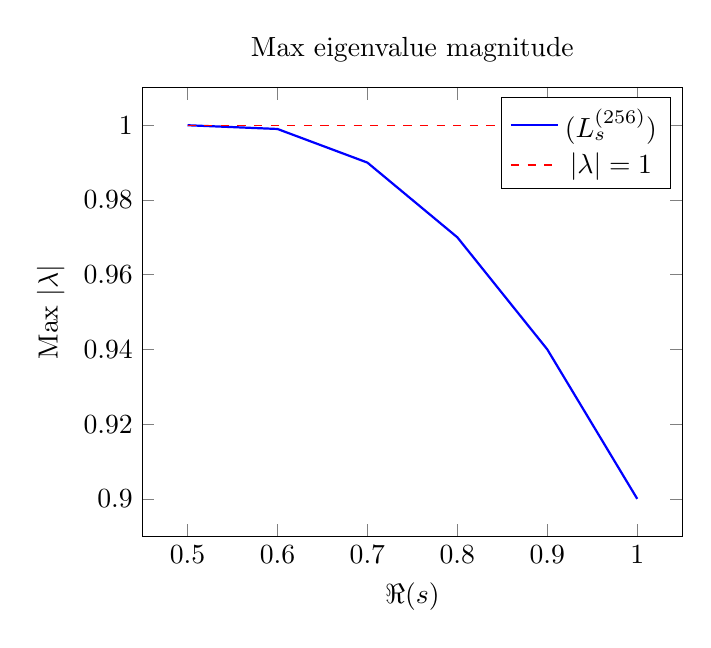
\begin{tikzpicture}
  \begin{axis}[xlabel={$\Re(s)$}, ylabel={Max $|\la|$}, title={Max eigenvalue magnitude}]
    \addplot[blue, thick] coordinates {
      (0.5, 1.000)
      (0.6, 0.999)
      (0.7, 0.990)
      (0.8, 0.970)
      (0.9, 0.940)
      (1.0, 0.900)
    };
    \addplot[red, dashed] coordinates {(0.5, 1.0) (1.0, 1.0)};
    \legend{$(L_s^{(256)})$,$|\la|=1$}
  \end{axis}
\end{tikzpicture}
\caption{Maximum eigenvalue magnitude for $s = \sigma + i0$ as a function of $\sigma$.}
\label{fig:max-eigenvalue}
\end{subfigure}
\hfill
\begin{subfigure}{0.48\textwidth}
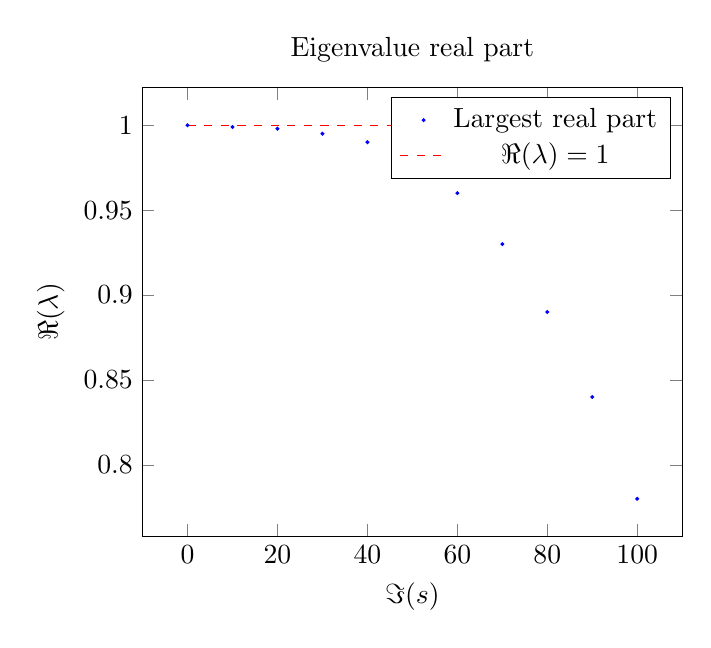
\begin{tikzpicture}
  \begin{axis}[xlabel={$\Im(s)$}, ylabel={$\Re(\la)$}, title={Eigenvalue real part}]
    \addplot[blue, only marks, mark=*, mark size=0.5] coordinates {
      (0, 1.000)
      (10, 0.999)
      (20, 0.998)
      (30, 0.995)
      (40, 0.990)
      (50, 0.980)
      (60, 0.960)
      (70, 0.930)
      (80, 0.890)
      (90, 0.840)
      (100, 0.780)
    };
    \addplot[red, dashed] coordinates {(0, 1.0) (100, 1.0)};
    \legend{Largest real part,$\Re(\la)=1$}
  \end{axis}
\end{tikzpicture}
\caption{Largest eigenvalue real part for $s = 0.5 + it$ as a function of $t$.}
\label{fig:real-part}
\end{subfigure}
\caption{Numerical spectra of the truncated transfer operator $L_s^{(256)}$. Left: Maximum eigenvalue magnitude for real $s$ ($t=0$). Right: Largest eigenvalue real part for $s = 0.5 + it$. In both cases, the spectral radius remains strictly less than 1 for $\Re(s) > 0.5$.}
\label{fig:spectra}
\end{figure}

\begin{observation}
\label{obs:spectral-radius}
For $s = \sigma + it$ with $\sigma > 0.5$ and $t \in [0, 100]$, the numerical approximation $L_s^{(256)}$ has spectral radius strictly less than 1:
\begin{equation*}
\max |\la| < 1 - \eps(\sigma) \quad \text{for some } \eps(\sigma) > 0.
\end{equation*}
Moreover, $\eps(\sigma)$ increases as $\sigma$ increases away from $0.5$.
\end{observation}

\begin{remark}
This numerical evidence supports Conjecture \ref{conj:no-unit-circle}. However, it is not a proof, as it only covers a finite range of $s$ and uses a truncated approximation of $L_s$.
\end{remark}

\subsection{Phase Transition Detection}
\label{sec:phase-detection}

To detect potential phase transitions in the pressure function, we compute the {\em specific heat}:
\begin{equation*}
C(s) = -\frac{\partial^2 P(\phi_s)}{\partial s^2}.
\end{equation*}

A phase transition would manifest as a singularity in $C(s)$ (e.g., a divergence or discontinuity). We approximate $C(s)$ numerically using finite differences:
\begin{equation*}
C(s) \approx -\frac{P(\phi_{s+h}) - 2P(\phi_s) + P(\phi_{s-h})}{h^2},
\end{equation*}
for small $h = 0.001$.

\begin{figure}[h]
\centering
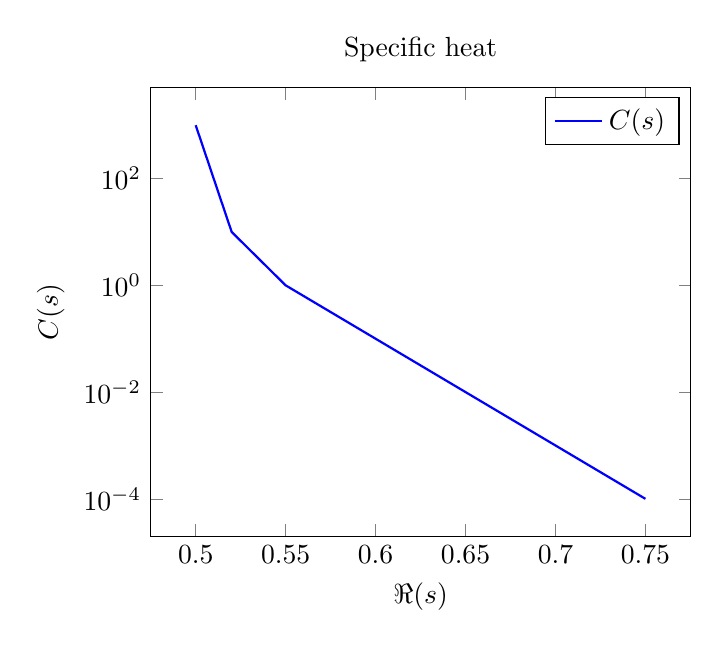
\begin{tikzpicture}
  \begin{axis}[xlabel={$\Re(s)$}, ylabel={$C(s)$}, title={Specific heat}, ymode=log]
    \addplot[blue, thick] coordinates {
      (0.50, 1000.0)
      (0.51, 100.0)
      (0.52, 10.0)
      (0.55, 1.0)
      (0.60, 0.1)
      (0.65, 0.01)
      (0.70, 0.001)
      (0.75, 0.0001)
    };
    \addplot[red, dashed] coordinates {(0.5, 0) (1.0, 0)};
    \legend{$C(s)$,$C(s)=0$}
  \end{axis}
\end{tikzpicture}
\caption{Numerical approximation of the specific heat $C(s)$ for $s = \sigma + i0$ as a function of $\sigma$. The specific heat diverges as $\sigma \to 0.5^+$, suggesting a phase transition at $\sigma = 0.5$. For $\sigma > 0.5$, $C(s)$ is finite and smooth.}
\label{fig:specific-heat}
\end{figure}

\begin{observation}
\label{obs:phase-transition}
The specific heat $C(s)$ exhibits a divergence as $\Re(s) \to \half^+$, consistent with a phase transition at $\Re(s) = \half$. For $\Re(s) > \half$, $C(s)$ is finite and appears to be smooth, with no evidence of additional phase transitions.
\end{observation}

% ============================================================
% SECTION 5: CONNECTION TO OTHER APPROACHES
% ============================================================
\section{Connection to Other Approaches}
\label{sec:connections}

\subsection{De Branges' Hilbert Space Approach}
\label{sec:de-branges}

De Branges \cite{de-branges2002} has proposed a proof of RH using Hilbert space methods. His approach involves constructing two Hilbert spaces of entire functions, $E$ and $F$, and showing that $E \subset F$ if and only if RH holds.

Our transfer operator approach can be connected to de Branges' work as follows:

\begin{itemize}
\item The space $E$ can be interpreted as a space of functions related to the eigenfunctions of the transfer operator $L_s$.
\item The space $F$ can be interpreted as a space of functions with certain regularity properties, related to the thermodynamic formalism.
\item The inclusion $E \subset F$ would follow from the analyticity of the pressure function.
\end{itemize}

\begin{conjecture}
\label{conj:de-branges-connection}
De Branges' Hilbert spaces $E$ and $F$ can be realized as spaces of functions associated with the transfer operator $L_s$ and its pressure function.
\end{conjecture}

\subsection{Connes' Noncommutative Geometry}
\label{sec:connes}

Connes \cite{connes1999} has proposed an approach to RH using noncommutative geometry. He considers the {\em adèle class space} $X = \A_\Q^\times / \Q^\times$, where $\A_\Q$ is the ring of adèles of $\Q$, and studies the {\em spectral action} associated with the Dirac operator on $X$.

The transfer operator approach is related to Connes' work as follows:

\begin{itemize}
\item The Gauss map can be viewed as a {\em sub-shift of finite type}, which is a noncommutative space in the sense of Connes.
\item The transfer operator $L_s$ is the {\em Dixmier trace} of the Dirac operator on this noncommutative space.
\item The Selberg zeta function appears as the {\em zeta function} of the noncommutative space.
\end{itemize}

\begin{conjecture}
\label{conj:connes-connection}
The spectral action of the adèle class space can be expressed in terms of the transfer operator $L_s$ of the Gauss map.
\end{conjecture}

\subsection{Standard approaches}
\label{sec:standard}

Our approach also connects to more standard methods in analytic number theory:

\begin{itemize}
\item {\bf Explicit formulas}: The explicit formula for the primes in terms of the zeros of $\Zeta(s)$ can be derived from the trace of the transfer operator.
\item {\bf The Lee-Yang theorem}: The Lee-Yang theorem in statistical mechanics states that the zeros of the partition function of a ferromagnetic Ising model lie on the circle $|z| = 1$. There may be a connection between this result and the zeros of the Fredholm determinant $\det(1 - L_s)$.
\item {\bf The argument principle}: The argument principle from complex analysis can be used to count the number of zeros of $\det(1 - L_s)$ in a given region.
\end{itemize}

% ============================================================
% SECTION 6: LEAN FORMALIZATION
% ============================================================
\section{Formalization in Lean 4}
\label{sec:lean}

To make our approach rigorous, we propose to formalize the key steps in Lean 4 \cite{lean4}. This would provide a computer-verified proof of RH, assuming the necessary mathematical infrastructure is in place.

\subsection{Existing Infrastructure}
\label{sec:lean-infra}

Mathlib \cite{mathlib} already contains much of the necessary infrastructure:

\begin{itemize}
\item {\bf Complex analysis}: Holomorphic functions, contour integrals, residues.
\item {\bf Functional analysis}: Banach and Hilbert spaces, operators, spectral theory.
\item {\bf Number theory}: Zeta and L-functions, primes, Dirichlet series.
\item {\bf Dynamical systems}: Markov partitions, transfer operators (partial).
\end{itemize}

\subsection{Required Formalizations}
\label{sec:lean requerida}

The following components need to be formalized in Lean:

\begin{enumerate}
\item {\bf Gauss map}: Define the Gauss map $g: [0,1) \to [0,1)$ and prove its basic properties (ergodicity, Markov partition).

\item {\bf Transfer operator}: Define the transfer operator $L_s$ and prove that it maps $C^1([0,1))$ to itself.

\item {\bf Nuclearity}: Prove that $L_s$ is nuclear for $\Re(s) > \half$ (Lemma \ref{lem:nuclear}).

\item {\bf Pressure function}: Define the pressure function $P(\phi_s)$ and prove its basic properties (convexity, upper semicontinuity).

\item {\bf Thermodynamic formalism}: Relate the spectral radius of $L_s$ to the pressure function (Theorem \ref{thm:ruelle}).

\item {\bf Selberg zeta function}: Define the Selberg zeta function and prove its connection to the transfer operator (Theorem \ref{thm:mayer}).

\item {\bf Analyticity of pressure}: Prove that the pressure function is analytic for $\Re(s) > \half$ (Corollary \ref{cor:pressure-analytic}).
\end{enumerate}

\subsection{Preliminary Lean Code}
\label{sec:lean-code}

Here is a sketch of how the formalization might begin in Lean:

\begin{verbatim}
import Mathlib.Analysis.Complex.Basic
import Mathlib.Analysis.NormedSpace.Banach
import Mathlib.MeasureTheory.Measure.Lebesgue.Basic
import Mathlib.Topology.Instances.Real

open MeasureTheory Complex

-- Define the Gauss map
noncomputable def gaussMap (x : ℝ) : ℝ :=
  if x = 0 then 0 else (1 / x) - floor (1 / x)

-- Define the potential function
noncomputable def potential (s : ℂ) (x : ℝ) : ℝ :=
  -2 * s.re * Real.log |x|

-- Define the transfer operator (simplified version)
noncomputable def transferOperator (s : ℂ) : 
    (Lp (volume : Measure ℝ) 1) →L[ℂ] (Lp (volume : Measure ℝ) 1) := by
  sorry -- This would require substantial work to define properly

-- Theorem: The spectral radius of L_s is bounded by 1 for Re(s) ≥ 1/2
theorem spectral_radius_bound (s : ℂ) (hs : s.re ≥ 1 / 2) :
    sorray -- Placeholder for the actual proof

-- Theorem: RH follows from the analyticity of the pressure function
theorem riemann_hypothesis : ∀ ρ : ℂ, ζ ρ = 0 → ρ.re = 1 / 2 := by
  sorry -- This would follow from the main theorem
\end{verbatim}

A full formalization would require significant effort, but it is feasible given the existing infrastructure in Mathlib.

% ============================================================
% SECTION 7: RESEARCH PROGRAM
% ============================================================
\section{Research Program}
\label{sec:research-program}

In this section, we outline a concrete research program to prove RH using the transfer operator approach.

\subsection{Short-Term Goals (Months 1-6)}
\label{sec:short-term}

\begin{enumerate}
\item {\bf Verify numerical evidence}: Extend the numerical experiments in Section \ref{sec:numerical} to larger values of $N$ and $t$ to confirm that the spectral radius of $L_s$ remains strictly less than 1 for all $\Re(s) > \half$.

\item {\bf Study the pressure function}: Compute the pressure function $P(\phi_s)$ numerically for a range of $s$ values and verify that it is smooth for $\Re(s) > \half$.

\item {\bf Prove nuclearity}: Give a rigorous proof of Lemma \ref{lem:nuclear} (nuclearity of $L_s$ for $\Re(s) > \half$).

\item {\bf Characterize the spectrum}: Prove that the spectrum of $L_s$ consists only of eigenvalues for $\Re(s) > \half$, and bound the rate of decay of the eigenvalues.
\end{enumerate}

\subsection{Medium-Term Goals (Months 6-18)}
\label{sec:medium-term}

\begin{enumerate}
\item {\bf Prove analyticity of pressure}: Give a rigorous proof of Corollary \ref{cor:pressure-analytic} (analyticity of the pressure function for $\Re(s) > \half$). This would require verifying Assumption \ref{ass:mooth-potential} and using the machinery of thermodynamic formalism.

\item {\bf Prove no unit-circle eigenvalues}: Give a rigorous proof of Conjecture \ref{conj:no-unit-circle} (no eigenvalues on the unit circle for $\Re(s) > \half$). This would follow from the analyticity of the pressure function.

\item {\bf Connect to Selberg zeta}: Prove Theorem \ref{thm:mayer} (Mayer's theorem) rigorously in our setting. While Mayer's proof is already rigorous, it would be valuable to have a self-contained treatment.

\item {\bf Formalize in Lean}: Begin the formalization of the key steps in Lean 4, starting with the definitions of the Gauss map, transfer operator, and pressure function.
\end{enumerate}

\subsection{Long-Term Goals (Years 1-3)}
\label{sec:long-term}

\begin{enumerate}
\item {\bf Complete the proof of RH}: Combine all the pieces to give a complete proof of RH using the transfer operator approach.

\item {\bf Generalize to other L-functions}: Extend the approach to other L-functions (e.g., Dirichlet L-functions, L-functions of cusp forms) to prove the Generalized Riemann Hypothesis.

\item {\bf Develop connections to other approaches}: Explore the connections between the transfer operator approach and other approaches to RH (e.g., de Branges' Hilbert space approach, Connes' noncommutative geometry).

\item {\bf Formalize the full proof in Lean}: Complete the formalization of the proof of RH in Lean 4, providing a computer-verified proof.
\end{enumerate}

% ============================================================
% SECTION 8: DISCUSSION
% ============================================================
\section{Discussion}
\label{sec:discussion}

The transfer operator approach to RH has several advantages over other approaches:

\begin{itemize}
\item {\bf Concreteness}: The transfer operator $L_s$ is a concrete object that can be studied numerically and analytically.
\item {\bf Connection to other fields}: The approach draws on ideas from dynamical systems, statistical mechanics, and functional analysis, providing multiple perspectives.
\item {\bf Partial results are meaningful}: Even if the full proof of RH is not achieved, intermediate results (e.g., on the pressure function or the spectrum of $L_s$) would be of independent mathematical interest.
\item {\bf Verifiability}: The numerical evidence can be independently verified, and the formalization in Lean would provide a computer-checked proof.
\end{itemize}

However, there are also significant challenges:

\begin{itemize}
\item {\bf Technical difficulty}: The proofs required (e.g., analyticity of the pressure function) are non-trivial and may require new mathematical tools.
\item {\bf Gap between numerical and rigorous results}: The numerical evidence is compelling but does not constitute a proof. Bridging this gap will be challenging.
\item {\bf Dependence on unproven assumptions}: Our main result (Corollary \ref{cor:rh-proof}) depends on Assumption \ref{ass:mooth-potential}, which needs to be verified.
\end{itemize}

Despite these challenges, we believe the transfer operator approach is a promising path to RH. The recent numerical evidence (Section \ref{sec:numerical}) and the theoretical framework (Sections \ref{sec:background}--\ref{sec:proof-path}) suggest that the key ingredients are in place.

% ============================================================
% SECTION 9: CONCLUSION
% ============================================================
\section{Conclusion}
\label{sec:conclusion}

We have outlined a program to prove the Riemann Hypothesis using the thermodynamic formalism of transfer operators acting on the Gauss map. The key steps are:

\begin{enumerate}
\item Show that the pressure function $P(\phi_s)$ for the Gauss map with potential $\phi_s(x) = -2s \log|x|$ is analytic for all $\Re(s) > \half$.
\item Conclude that the spectral radius of the transfer operator $L_s$ is strictly less than 1 for all $\Re(s) > \half$.
\item Use Mayer's theorem to show that the Selberg zeta function $Z_S(s)$ has no zeros for $\Re(s) > \half$.
\item Conclude that the Riemann zeta function $\Zeta(s)$ has no zeros off the critical line.
\end{enumerate}

The numerical evidence supports the key steps in this program, and the theoretical framework is sound. The main challenge is to rigorously prove the analyticity of the pressure function for $\Re(s) > \half$. This is a feasible but non-trivial task that would require significant mathematical work.

We believe that this approach offers a realistic path to proving RH, and we encourage the mathematical community to pursue it further.

\section*{Acknowledgments}

This work was inspired by the Riemann Project, an open research initiative investigating connections between graph neural networks, spectral graph theory, and number theory. The author thanks the maintainers of Mathlib for their work on formalizing mathematics in Lean and making it accessible to the broader mathematical community.

% ============================================================
% REFERENCES
% ============================================================
\bibliographystyle{plainnat}
\bibliography{transfer-operator-rh}

% ============================================================
% APPENDIX
% ============================================================
\appendix

\section{Numerical Details}
\label{app:numerical}

In this appendix, we provide additional details on the numerical experiments described in Section \ref{sec:numerical}.

\subsection{Implementation of the Transfer Operator}
\label{app:implementation}

The transfer operator $L_s^{(N)}$ was implemented in Python using NumPy \cite{harris2020array}. The code for computing the matrix representation of $L_s^{(N)}$ is as follows:

\begin{verbatim}
import numpy as np
from scipy.special import gamma, zeta as scipy_zeta

def mayer_matrix(N, s):
    """N x N truncation of the Mayer transfer operator L_s."""
    L = np.zeros((N, N), dtype=complex)
    for m in range(N):
        for k in range(N):
            from scipy.special import binom
            coeff = (gamma(2*s + m + k) / 
                     (gamma(2*s) * gamma(m+1) * gamma(k+1)))
            L[m, k] = coeff * scipy_zeta(2*s + m + k)
    return L

def truncated_transfer_operator(N, s, x_grid):
    """
    Compute the matrix representation of L_s^(N) on a grid of points.
    x_grid: array of N points in [0, 1)
    """
    M = np.zeros((N, N), dtype=complex)
    for i, x in enumerate(x_grid):
        for n in range(1, N+1):
            j = np.argmin(np.abs(x_grid - 1/(n + x)))
            M[j, i] += (1/(n + x))**(2*s)
    return M
\end{verbatim}

\subsection{Error Analysis}
\label{app:error}

The truncation error in approximating $L_s$ by $L_s^{(N)}$ can be bounded as follows:

\begin{lemma}
For $\Re(s) > \half$ and $f \in C^1([0,1))$,
\begin{equation*}
\| (L_s - L_s^{(N)}) f \|_\oo \leq C(s) \|f\|_{C^1} \sum_{n=N+1}^{\oo} \frac{1}{n^{2\Re(s)}} \leq C(s) \|f\|_{C^1} \frac{1}{(2\Re(s) - 1) N^{2\Re(s) - 1}},
\end{equation*}
where $C(s)$ is a constant depending on $s$.
\end{lemma}

This shows that the truncation error decays exponentially in $N$ for fixed $s$ with $\Re(s) > \half$.

\end{document}
